\subsection{Extensible Data Acquisition Tool} \label{background:svein}
In the thesis "Extensible data acquisition tool for Android" by Gjøby \cite{gjoby} a proposition of a \textit{data acquisition system} for Android is presented. The thesis proposes a system that hides the low-level sensor-specific details into two components, \textit{providers} and \textit{sensor wrappers}. The provider is responsible for the functionality that is common for all data sources (e.g., starting and stopping the data acquisition), while the sensor wrapper is responsible for the data source specific functionality (e.g., communicating with the data source).

The thesis solves the difficulties around creating an extensible data acquisition tool, connecting new and existing sensors, and finding a common interface. The problem statement of the thesis addresses the following concerns regarding sensors:
\begin{itemize}
    \item \textit{Common abstraction/interface for the interchanged data}\\ 
    Sensor platform manufacturers have their low-level protocol to support the functionality of their product. Typically, the manufacturers provide software development kits (SDKs) to hide the low-level protocols so third-party developers can be easier; however, both the low-level protocol and the SDKs are not standardized. Thus, for each sensor, there might be different commands and methods.
    \item \textit{Various Link Layer technologies} \\ 
    Each sensor might use different Link Layer technology (i.e., Ethernet, USB, BlueTooth, WiFi, ANT+, and ZigBee), which means establishing a connection between a device and a sensor might differ. For instance, BlueTooth devices need to be paired, while devices on the WiFi can address each other without any pairing. 
    \item \textit{Reusability of sensor code}\\
    Applications that implement support for the low-level protocol of a sensor type can not be shared between different applications. Thus, introducing duplicate work and code if multiple application wish to use the same sensor type. A framework that isolates the sensor that applications can use, might make it easier for application to utilize the collected data. In addition, isolating the sensors into modules improves the robustness and quality of the implementation. 
    
\end{itemize}

In the thesis, the goal is to develop an extensible system, which enables applications to collect data from various external and built-in sensors through one common interface. The solution around an extensible system is to have the core of the application unchangeable when adding support for a new data source, regardless of the Link Layer technology and communication protocol used by the data source. Making all the data sources behave as the same, is a naive solution to the problem. However, separating the software into two different components, a \textit{provider} component and a \textit{sensor wrapper} component, enables the reuse of functionality that is common amongst the data sources. 

The sensor wrapper application is tailored to suit the Link Layer technology and data exchange protocol of one particular data source. Additionally, responsible for connectivity and communication with the data source. The provider application is responsible for managing the sensor wrappers---starting and stopping the data acquisition---and processing the data received from the sensor wrapper application. Thus, everything that is independents of the data source should be a part of the provider application. With this type of solution, the possibility to reuse the sensor wrapper application for different provider applications is made possible. However, there are some overheads with this solution. Mostly, the inter-process communication that might be costly and increase the complexity of the code. Nonetheless, the flexibility and extensibility gained by separating the functionalists out weights the cost.

When a connection is established with the provider application, a package of metrics and data type (all the data does not change during the acquisition as metadata) is sent describing the context of the data collected. The metadata is necessary because different sensors might sample data in different environments, and some applications are depending on recognizing the environment of the data acquisition. Therefore, it is critical to know what data values are measured. Consequently, exposing sensors and data channels through one common interface requires a field of metadata which can be used to: (1) \textit{distinguish} sensor wrapper and data channel the data originated from; (2) determine the \textit{capabilities} of the sensors (i.e., EEG, ECG, LUX); (3) determine the \textit{unit} the data is represented in (i.e., for temperature, Celsius or Fahrenheit); (4) describing the data channel (i.e., placement of the sensor); and (5) a timestamp of when the data was sampled. 

To summarize, the task of a \textit{sensor wrapper} is to establish a connection to and collect data from precisely one specified data source, and to send the collected data to the \textit{provider application} that is listening for it. A data source (e.g., BiTalion) can have support for multiple sensor attachments (defined as data channel in the thesis), although, only on sensor wrapper is necessary for each data source and their data channels. Each sensor wrapper is tailored to adapt to the data source's Link Layer technology and the communication protocol of a respective data source. Upon activation by a provider application, the data is collected by the sensor wrapper, and pushed to the provider application in a JSON-format. An illustration of the structure is found in Figure \ref{fig:provider_SW}.

\begin{figure}
    \centering
    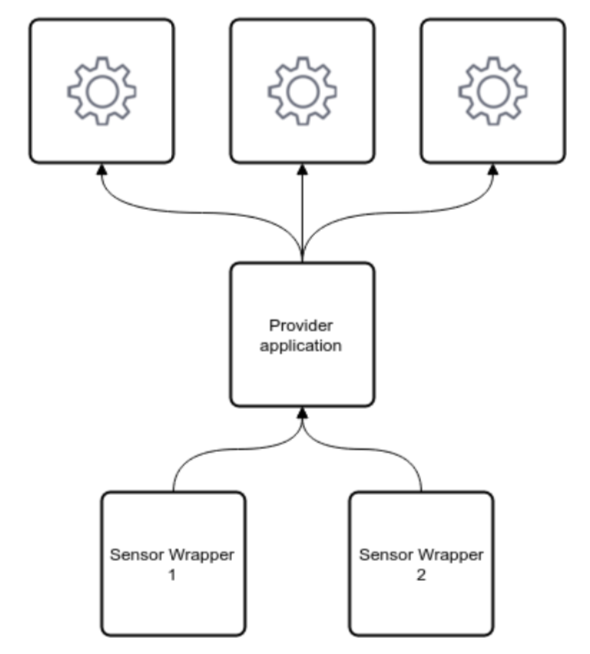
\includegraphics[width=0.5\textwidth]{images/provider_SW.png}
    \caption{Sharing the collected data between multiple applications \cite{gjoby}}
    \label{fig:provider_SW}
\end{figure}
\subsection{Extensible Data Streams Dispatching Tool}\label{background:daniel}
The extensible data acquisition tool developed by Gjøby leaves some space for improvements. Such improvements are discussed in the thesis "Extensible data streams dispatching tool for Android" by Bugajski \cite{daniel}. The thesis analyses the potential improvements of the data acquisition tools, which can be extracted into:
\begin{itemize}
    \item \textit{Lack of reusability} \\ Only the components that have started the collection can receive the data, and no other components can access the collected data.
    \item \textit{Lack of sharing} \\ Components that perform specific analysis on the collected data in real-time have no way of share the results of the analysis such that other components can use them. 
    \item \textit{Lack of tuning} \\ It is not allowed to change the frequency of collection after the start. Thus, the user has to stop the collection and manually change the frequency of the sensor and then restart the collection. 
    \item \textit{Lack of customization} \\ The set of channels cannot be changed during a collection, and the collector receives data from all channels even if it needs only one of them. Thus, the data packet size and resource usage become larger than necessary.
\end{itemize}

In the thesis, the modularity of the architecture is improved by finding a common model for all available data channels, developing a mechanism for cloning a data packet to allow reusing of data across modules, and allowing the modules to have support for choosing channels they want to receive data from and publish their data to. In the model, these components are distinguished as: 
\begin{enumerate}
    \item \textit{sensor-capability model}: is a representation of all distinct data types and contains all information about the channel. A sensor board usually reads and sends different type of data to a mobile device. Thus, this module is used to control every available data type, such that they can be accessed from the application part at any time.
    \item \textit{demultiplexer} (DMUX): is a data cloner, that receives data packets from one input (e.g., from one channel), and duplicates the data several times based on the number of subscribers.
    \item \textit{publish-subscribe} mechanism: is an interface responsible for managing requests from subscribers or publishers, also, to be able to terminate these statuses. Additionally, every module from the application will be able to see all capabilities represented by this component, enabling the option to choose a frequency the data collection.
\end{enumerate}

\begin{figure}
    \centering
    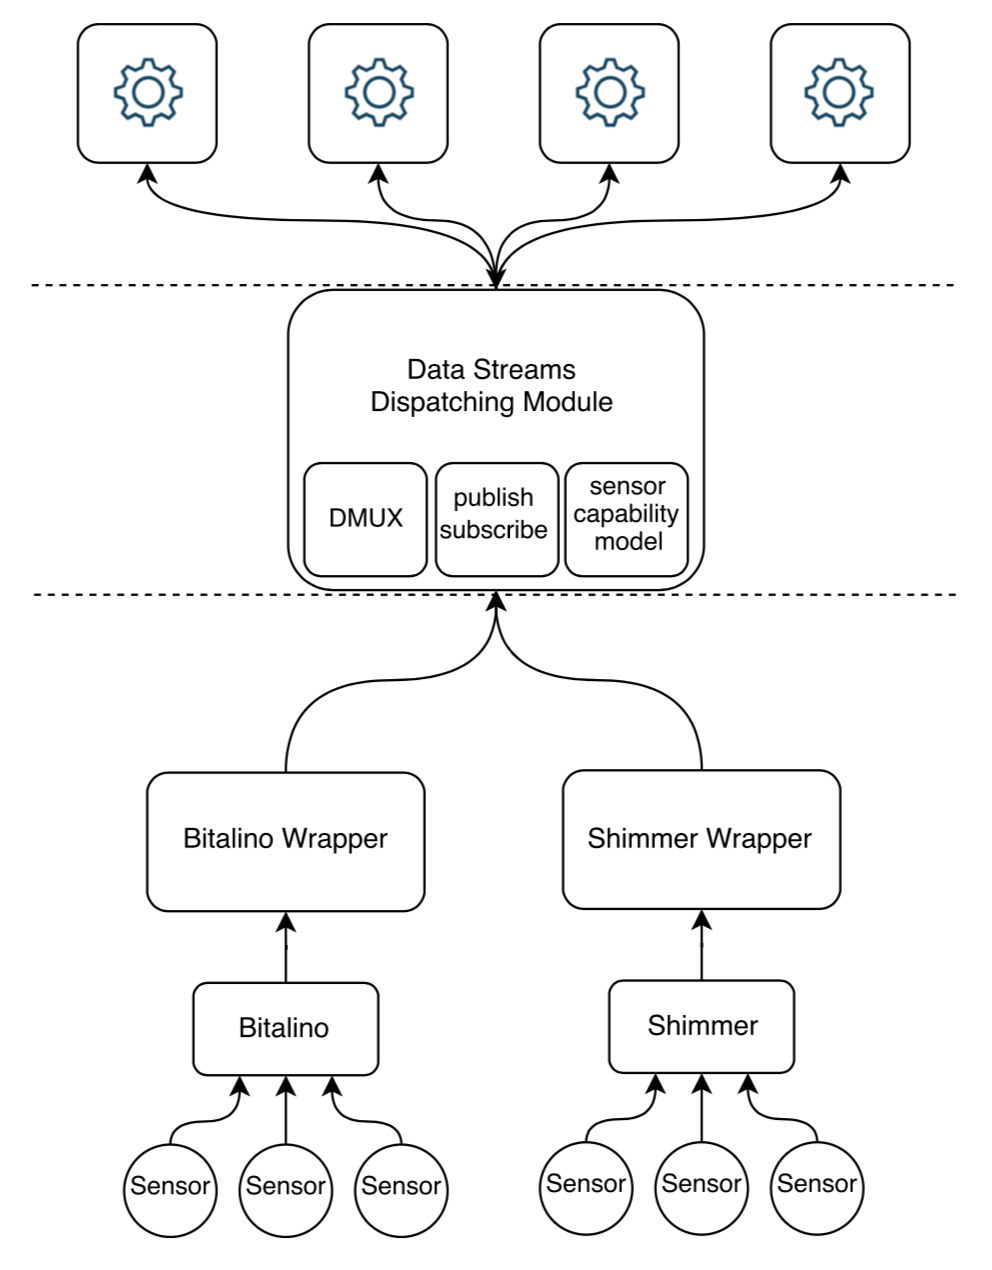
\includegraphics[width=0.65\textwidth]{images/demux.png}
    \caption{Sharing the collected data between multiple applications \cite{daniel}}
    \label{fig:demux}
\end{figure}

The combination of how these modules cooperate and communicate with each other affects the modularity and performance of the architecture. In the thesis, there are various proposed solutions. The naive solution was to fit all of the elements into each respective sensor wrapper, thus, prioritizing the performance and low resource usage, but making it impossible to distinguish data type from two sensor wrapper with the same data type. This is optimal for the cases where collection only occurs on one sensor board. An improved solution includes to place the demux between the application part and the wrapper layer and to insert the remaining elements in the respective application part. This solution resolves the overload of sensor wrappers performing other tasks besides collecting data; thus, the wrappers are untouched, and they send the data to the demux. However, there are several issues with this solution, e.g., due to various obstacles such as (1) every application module has to configure its sensor-capability model; (2) filter requested data packets from all the channels; (3) and deal with the collection speed on its own.

Addressing these issues leads to the final architecture, which is presented in Figure \ref{fig:demux}, and meets the demands identified in the requirements. In this solution, all elements are placed between the application part and the wrapper layer, forming the data stream dispatching module. The sensor wrapper connects directly to the data streams dispatching module; the module discovers all installed wrappers and populates the sensor-capability model with the data types from all installed sensors. By this, all applications can access a shared sensor-capability mode. A publish-subscribe mechanism enables application modules to subscribe to any capabilities with a preferred sampling rate. Correspondingly, an application module can publish data to other applications through the same interface. The demultiplexing element creates for each subscriber a copy of the data packet. 

To summarize, these three elements together establish \textit{the data stream dispatching module}. The final architecture has a couple of advantages, such as it is exceedingly extensible due to its maintainability. For instance, all communication with other layers occurs through one interface; this way, new instances can be added at any time, without the need for modifying large parts of the system. The system is also efficient due to packets are immediately sent to the application on request (without any buffers), and packets are only sent to the application requesting them, resulting in less resource and power usage, and more battery life. This tool is an improvement to Gjøby's solutions due to these facts.


\subsection{Flow Sensor Kit}
Flow is an activity sensor created by SweetZpot Inc., initially designed for measuring breathing and heart rate during activities. The sensor measures breathing per minute, in correlation to the heart rate, for optimal activity measurement. As stated on their page: \textit{"usually, at rest, your breathing varies between 6 and 8 liters per minute. During sleep, breathing can be as low as 3 liters per minute and can reach 160 liters per minute and above during high-intensity athletic activity"} \cite{flow}. Thus, this sensor could be suiting for measuring sleeping problems in the project.

The sensor is a  strap-on placed beneath the chest. It weighs 27 grams and dimensions of 77x43x17mm. Additionally, it is equipped with a 3V Lithium battery, with an estimated battery life of one year (with 7 hours a weekly usage). The sensor can be connected with BlueTooth technology, making it possible to connect with a mobile device.